\documentclass[12pt,letterpaper]{hmcpset}
\usepackage[margin=1in]{geometry}
\usepackage{graphicx}
\usepackage{hyperref}

% info for header block in upper right hand corner
\name{Name: \underline{\hspace{4cm}}}
\class{Math 45: Section \underline{\hspace{1cm}}}
\assignment{Assignment 5}
\duedate{4/13/18}

\begin{document}

\begin{problem}
1: (5 points) Consider the general, linear, second-order, constant-coefficient, homogeneous differential
equation $ay'' + by' + cy = 0$. Assuming a $\neq$ 0, if we divide the whole equation by a,
we arrive at

\begin{center}
    $y'' + \alpha y' + \beta y = 0.$
\end{center}
where $\alpha = b/a$ and $\beta = c/a$. Assume that $\alpha$ and $\beta$ are real numbers.

\begin{enumerate}
    \item[(a)] For which values of $\alpha$ and $\beta$ will we get solutions that oscillate (i.e., the roots of the
characteristic equation are complex)? For which values of $\alpha$ and $\beta$ will we get solutions
that don’t oscillate? For which values of $\alpha$ and $\beta$ will we get repeated roots of the
characteristic equation?
    \item[(b)] You saw before on homework 4 what values of $\lambda$ must be to get solutions that decay
to zero as $t \rightarrow \infty$. Now answer for what values of $\alpha$ and $\beta$ will we get solutions that
decay to zero as $t \rightarrow \infty$? For which values of $\alpha$ and $\beta$ will we get solutions that grow
exponentially (oscillatory or not) as $t \rightarrow \infty$?
    \item[(c)] Draw a plane with $\alpha$ and $\beta$ as the two axes. Summarize the information in parts (a)
and (b) graphically by showing which regions of the plane correspond to different types
of behaviors.
    \item[(d)] Watch this video: 
    \url{http://vimeo.com/63064216}. 
    If the behavior of the door could be
described by a linear, second-order, constant-coefficient, homogeneous ODE, what must
be true about the parameters $\alpha$ and $\beta$?
\end{enumerate}

\end{problem}
\newpage

\begin{problem}
2: (5 points) Consider the IVP $y'' - 4y' + 4y = 2x$ with $y(0) = 5$, $y'(0) = 3$.

\begin{enumerate}
    \item[(a)] Use the method of variation of parameters find the solution to this IVP.
    \item[(b)] Now use the method of undetermined coefficients to find the solution to this IVP.
(You do not have to redo the part where find the unknown constants using the initial
conditions—you can reuse your work from the previous part.)
\end{enumerate}
\end{problem}
\newpage

\begin{problem}
3: (5 points) Consider the DE $y'' + 3y' + 2y = e^{-2x}$.

\begin{enumerate}
    \item[(a)] Use the method of variation of parameters find the general solution to this DE.
    \item[(b)] Now use the method of undetermined coefficients to find the general solution.
    \item[(c)] If your two solutions from part (a) and part (b) are different, reconcile them.
\end{enumerate}
\end{problem}
\newpage

\begin{problem}
4: (10 points; 5 points for (a) and 5 points for (b)) For each IVP below, think about whether undetermined coefficients or variation of parameters would be more desirable to use. Solve using whichever method you think is best.
\begin{enumerate}
    \item[(a)] $y'' - 2y' + y= \frac{e^t}{1+t^2}$ with $y(0) = y'(0)=0$
    \item[(b)] $y'' +  y= 10e^{2t}$ with $y(0) = y'(0)=0$
\end{enumerate}

\end{problem}
\newpage

\begin{problem}
5: (5 points) Use the Wronskian to determine whether the following functions $y_1$ and $y_2$ are
linearly independent or linearly dependent on the interval $t \in (0, 1)$.
\begin{enumerate}
    \item[(a)] $y_1(t) = e^{5t}, y_2(t) = e^{-3t}$
    \item[(b)] $y_1(t) = t^2, y_2(t) = t^4$
    \item[(c)] $y_1(t) = \text{cos}(t) \text{sin}(t) = \text{sin}2t$
    \item[(d)] $y_1(t) = e^{\alpha t}\text{cos}(\beta t), y_2(t) = e^{\alpha t}\text{sin}(\beta t)$ ($\alpha$, $\beta$ constants, $\beta \neq 0$)
\end{enumerate}
\end{problem}
\newpage

\begin{problem}
6: (5 points) Consider the equation
\begin{center}
    $y'' + p(t)y' + q(t)y = 0$, $t \in I$
\end{center}
where $p(t)$ and $q(t)$ are continuous on $I$. Let $y_1$ and $y_2$ be solutions to this equation.
\begin{enumerate}
    \item[(a)] Prove that if $y_1$ and $y_2$ are zero at the same point in $I$, then they cannot be a \textit{fundamental solution set} (i.e. basis for the set of solutions) on $I$.
    \item[(b)] Prove that if $y_1$ and $y_2$ have maxima or minima at the same point in $I$, then they cannot be a \textit{fundamental solution set} on $I$.
\end{enumerate}
\end{problem}
\newpage

\begin{problem}
7: (5 points) Examine Student R's work on the following problem. What did the student do
correctly? What mistake(s) did the student make? (There are at least three.) What is a more
correct response to the problem, and what would you say to help the student understand
how to correctly complete the problem?

\begin{center}
$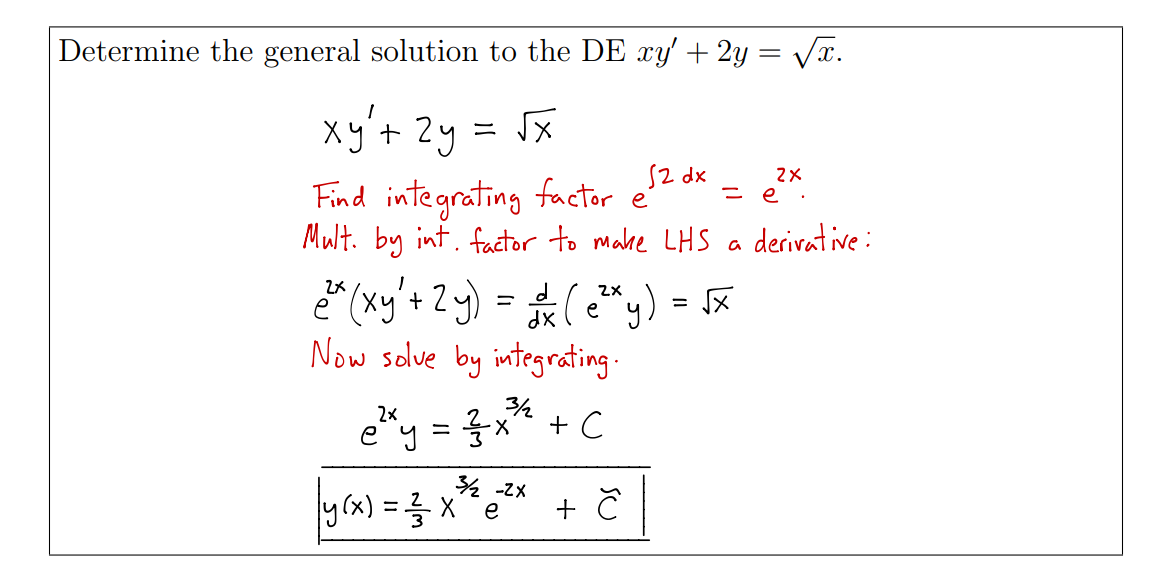
\includegraphics[scale=.4]{StudentR.png}$
\end{center}

\end{problem}
\newpage

\begin{problem}
8: (5 points) Meet with your project groups sometime before class Friday to discuss what
you want to model. Be prepared to discuss your model on Friday. Each member of
your group must sign your homework to verify that you met. Here are important guidelines
you can follow when collaborating:
\url{https://drive.google.com/drive/u/0/folders/
17p6TQosy900yKBUCWqMlvws-cOAmyCex}


\end{problem}
\newpage

\end{document}
